% Report skeleton for SMML Assignment 3 -- Regularization and Stability.
% The prose is YOURS to write: every section below contains only a TODO comment
% pointing to the matching section of report/NOTES.md (facts and numbers).
% Compile on Overleaf (upload the whole repo, or this folder plus ../figures)
% or locally with:  cd report && pdflatex main && bibtex main && pdflatex main && pdflatex main
% Target length: 5-10 pages.

\documentclass[11pt,a4paper]{article}
\usepackage[utf8]{inputenc}
\usepackage[T1]{fontenc}
\usepackage[margin=2.5cm]{geometry}
\usepackage{amsmath,amssymb}
\usepackage{graphicx}
\usepackage{booktabs}   % needed by figures/summary_table.tex
\usepackage{caption}
\usepackage{hyperref}
\graphicspath{{../figures/}}

\title{Regularization and Stability:\\an Empirical Study of Ridge Regression}
\author{Precious Prince\\Statistical Methods for Machine Learning, A.Y.\ 2025/26\\Universit\`a degli Studi di Milano}
\date{\today}

\begin{document}
\maketitle

% ---------------------------------------------------------------------------
\begin{abstract}
% TODO (you): 4-6 sentences: question, method, the three main findings. See NOTES.md "Abstract".
\end{abstract}

% ---------------------------------------------------------------------------
\section{Introduction}
% TODO (you): motivation and research questions. See NOTES.md "1 Introduction".
% Cite the paper as \cite{bousquet2002stability}.

% ---------------------------------------------------------------------------
\section{Background}
\subsection{Algorithmic stability}
% TODO (you): define S, S^{\setminus i}, uniform stability, and the bound. See NOTES.md "2.1".

\subsection{Ridge regression and why it is stable}
% TODO (you): objective, normal equations, eigenvalue argument, Sherman--Morrison identity. See NOTES.md "2.2".
% Useful equations (already typeset for you to keep or edit):
% \begin{equation}
%   \hat w = \arg\min_w \frac{1}{n}\sum_{i=1}^n (y_i - w^\top z_i)^2 + \lambda\|w\|^2
%          = (Z^\top Z + n\lambda I)^{-1} Z^\top y
% \end{equation}
% \begin{equation}
%   w_S - w_{S^{\setminus i}} = (Z^\top Z + n\lambda I)^{-1} z_i \,\bigl(y_i - f_{S^{\setminus i}}(x_i)\bigr)
% \end{equation}

% ---------------------------------------------------------------------------
\section{Datasets}
% TODO (you): synthetic generator and Diabetes; why these sizes; conditioning. See NOTES.md "3".

% ---------------------------------------------------------------------------
\section{Implementation}
% TODO (you): from-scratch models, standardisation inside fit, LOO refits, the three metrics,
% testing strategy. See NOTES.md "4".

% ---------------------------------------------------------------------------
\section{Experimental setup}
% TODO (you): lambda grid, repetitions, seeds, runs A--D. See NOTES.md "5".

% ---------------------------------------------------------------------------
\section{Results}

\begin{figure}[ht]
  \centering
  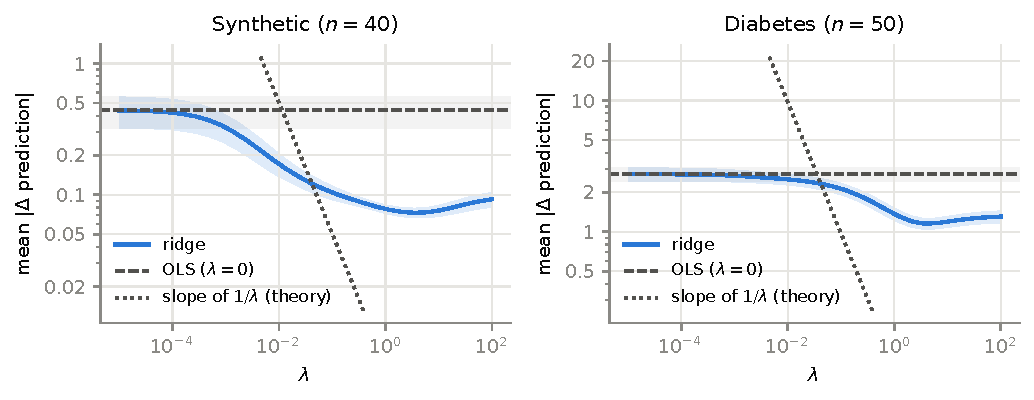
\includegraphics[width=\linewidth]{fig1_stability_vs_lambda.pdf}
  \caption{% TODO (you): caption. See NOTES.md "6 / Figure 1".
  }
  \label{fig:stab-lambda}
\end{figure}

\begin{figure}[ht]
  \centering
  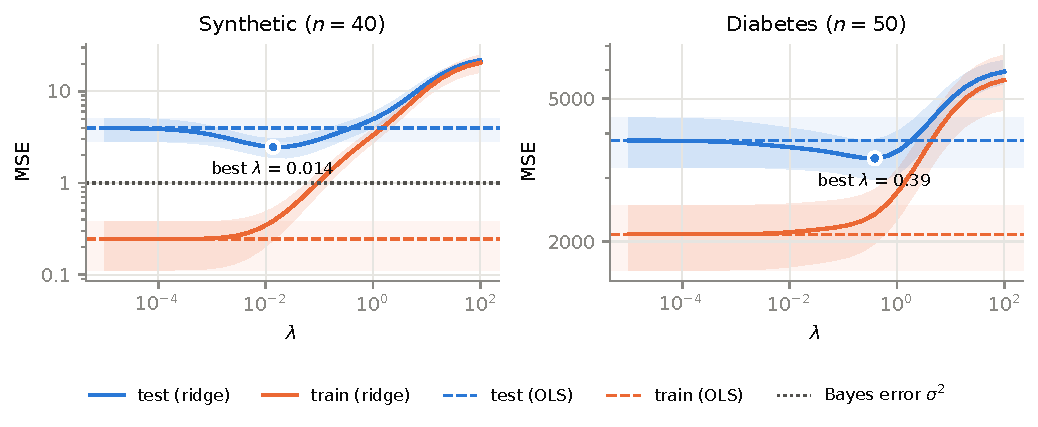
\includegraphics[width=\linewidth]{fig2_error_vs_lambda.pdf}
  \caption{% TODO (you)
  }
  \label{fig:err-lambda}
\end{figure}

\begin{figure}[ht]
  \centering
  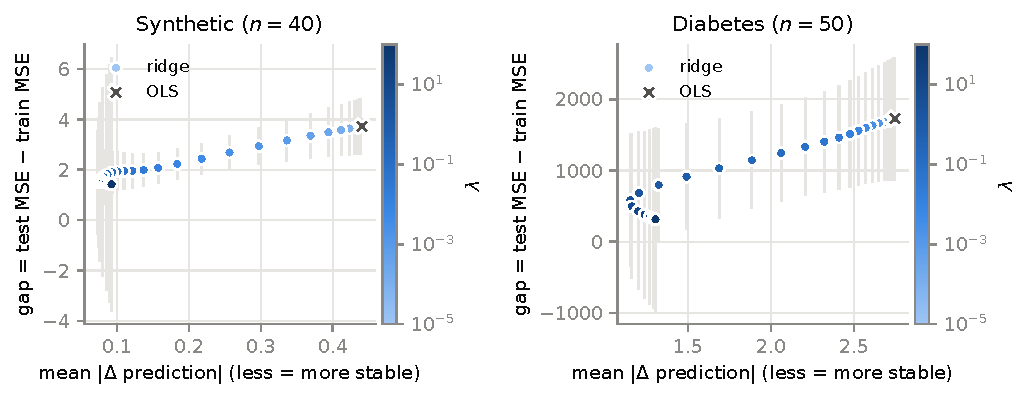
\includegraphics[width=\linewidth]{fig3_stability_vs_gap.pdf}
  \caption{% TODO (you)
  }
  \label{fig:stab-gap}
\end{figure}

\begin{figure}[ht]
  \centering
  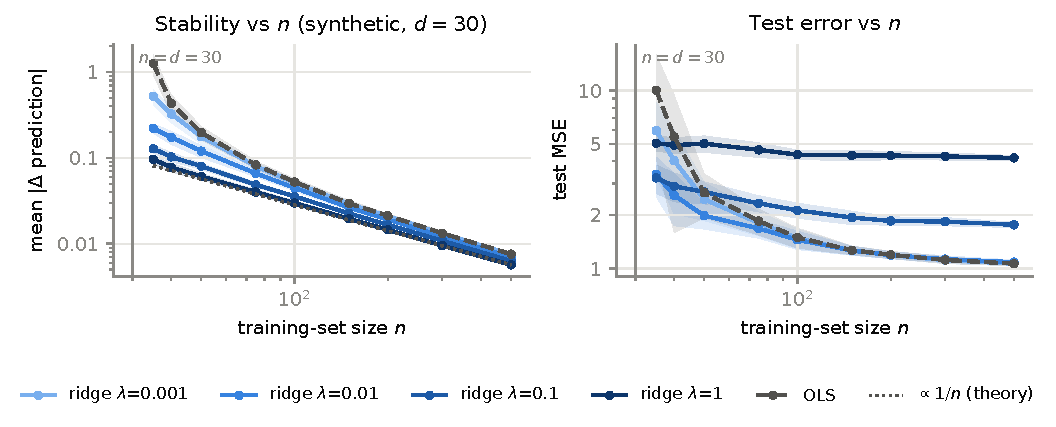
\includegraphics[width=\linewidth]{fig4_size_sweep.pdf}
  \caption{% TODO (you)
  }
  \label{fig:size}
\end{figure}

\begin{figure}[ht]
  \centering
  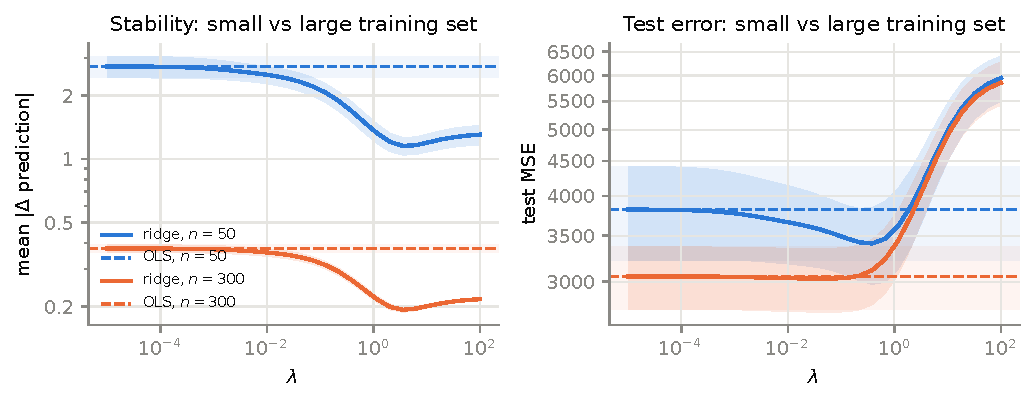
\includegraphics[width=\linewidth]{fig5_contrast_diabetes.pdf}
  \caption{% TODO (you)
  }
  \label{fig:contrast}
\end{figure}

\begin{figure}[ht]
  \centering
  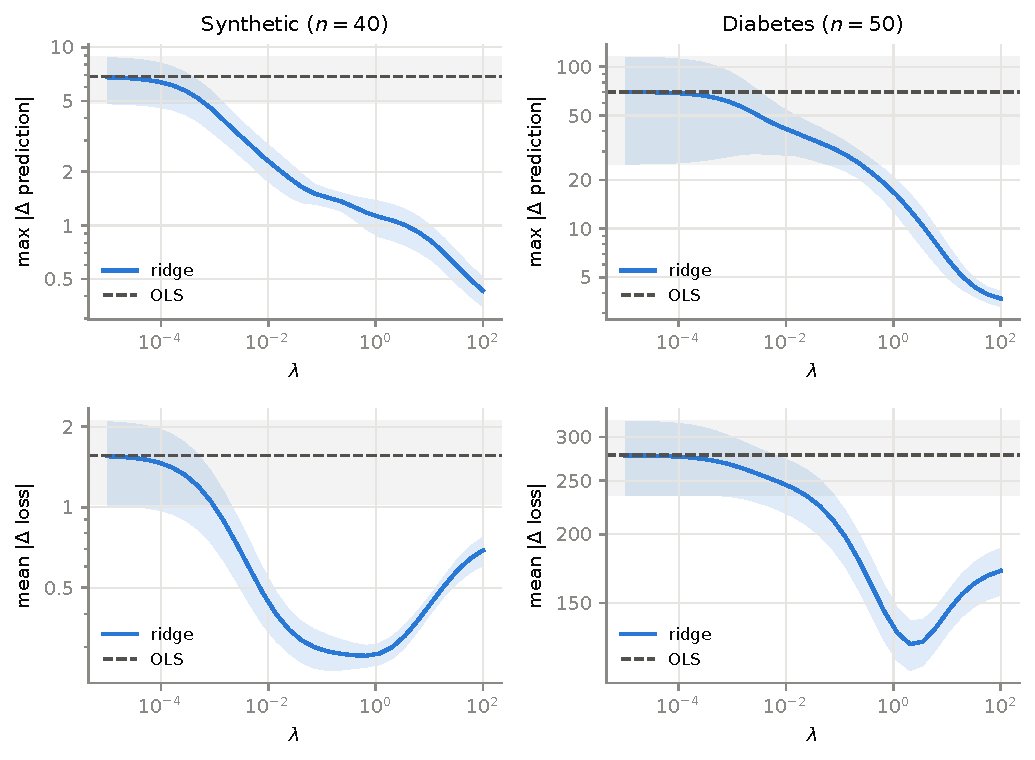
\includegraphics[width=0.8\linewidth]{fig6_metric_agreement.pdf}
  \caption{% TODO (you)
  }
  \label{fig:metrics}
\end{figure}

\begin{table}[ht]
  \centering
  \small
  \begin{tabular}{llrrrrrr}
\toprule
Dataset & Model & $\lambda$ & Train MSE & Test MSE & Gap & Stability & Test $R^2$ \\
\midrule
Synthetic & OLS & 0 & 0.244 $\pm$ 0.13 & 3.97 $\pm$ 1.1 & 3.73 $\pm$ 1.1 & 0.441 $\pm$ 0.12 & -- \\
Synthetic & Ridge (best $\lambda$) & 0.014 & 0.383 $\pm$ 0.15 & 2.46 $\pm$ 0.58 & 2.08 $\pm$ 0.61 & 0.157 $\pm$ 0.029 & -- \\
Diabetes ($n=50$) & OLS & 0 & 2.1e+03 $\pm$ 4.3e+02 & 3.82e+03 $\pm$ 6e+02 & 1.73e+03 $\pm$ 8.6e+02 & 2.75 $\pm$ 0.32 & 0.36 $\pm$ 0.11 \\
Diabetes ($n=50$) & Ridge (best $\lambda$) & 0.39 & 2.38e+03 $\pm$ 4.1e+02 & 3.41e+03 $\pm$ 4.4e+02 & 1.03e+03 $\pm$ 7e+02 & 1.69 $\pm$ 0.19 & 0.43 $\pm$ 0.057 \\
Diabetes ($n=300$) & OLS & 0 & 2.82e+03 $\pm$ 1.5e+02 & 3.05e+03 $\pm$ 3.2e+02 & 233 $\pm$ 4.7e+02 & 0.376 $\pm$ 0.016 & 0.49 $\pm$ 0.038 \\
Diabetes ($n=300$) & Ridge (best $\lambda$) & 0.042 & 2.85e+03 $\pm$ 1.5e+02 & 3.03e+03 $\pm$ 3.2e+02 & 184 $\pm$ 4.7e+02 & 0.342 $\pm$ 0.015 & 0.49 $\pm$ 0.036 \\
\bottomrule
\end{tabular}

  \caption{% TODO (you): OLS vs best-$\lambda$ ridge, mean $\pm$ std over 20 repetitions.
  }
  \label{tab:summary}
\end{table}

% TODO (you): describe each figure/table in the text. See NOTES.md "6".

% ---------------------------------------------------------------------------
\section{Discussion}
% TODO (you): link to the theory; positive AND negative aspects. See NOTES.md "7".

% ---------------------------------------------------------------------------
\section{Conclusion}
% TODO (you): See NOTES.md "8".

\bibliographystyle{plain}
\bibliography{refs}

% ---------------------------------------------------------------------------
\section*{Declaration}
I declare that this material, which I now submit for assessment, is entirely my own work and has not been taken from the work of others, save and to the extent that such work has been cited and acknowledged within the text of my work. I understand that plagiarism, collusion, and copying are grave and serious offences in the university and accept the penalties that would be imposed should I engage in plagiarism, collusion or copying. This assignment, or any part of it, has not been previously submitted by me or any other person for assessment on this or any other course of study.

\end{document}
